Nesta seção, será tomado como exemplo a relação de corrente e tensão em um resistor, dado pela teoria por (\ref{eq:resist}). São os mesmos dados da figura \ref{fig:basico:importado}, da seção \nameref{sec:basico}, que foram gerados por computador.

\begin{equacao} \label{eq:resist}
    I = \frac{1}{R} ~ V
\end{equacao}

Por mais que sejam esses os dados usados aqui, essa parte de apresentação de dados é importante para todos dados, em especial, quando coletados à mão, como é o caso dos experimentos da disciplina de \texttt{F 329}.


\subsection{Dados Pontuais}

    Normalmente, quando se trata de dados pontuais, é importante mostrar esses dados em alguma tabela e no gráfico também. O modo de se fazer isso no \texttt{Origin} é com a funcionalidade \texttt{Scatter} (figura \ref{fig:reta:scatter}).

    \begin{figure}[htbp]
        \centering
        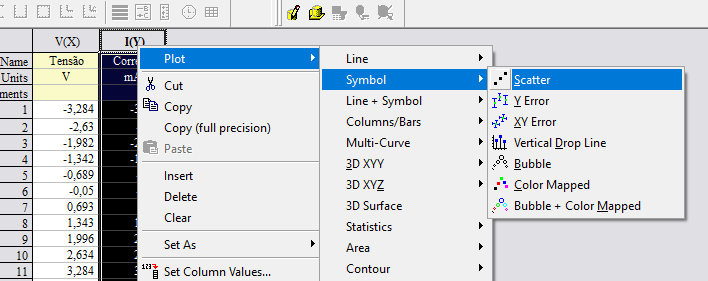
\includegraphics[width=0.7\textwidth]{reta/1scatter.png}

        \caption{\texttt{Scatter}}
        \label{fig:reta:scatter}
    \end{figure}

    \begin{figure}[htbp]
        \centering
        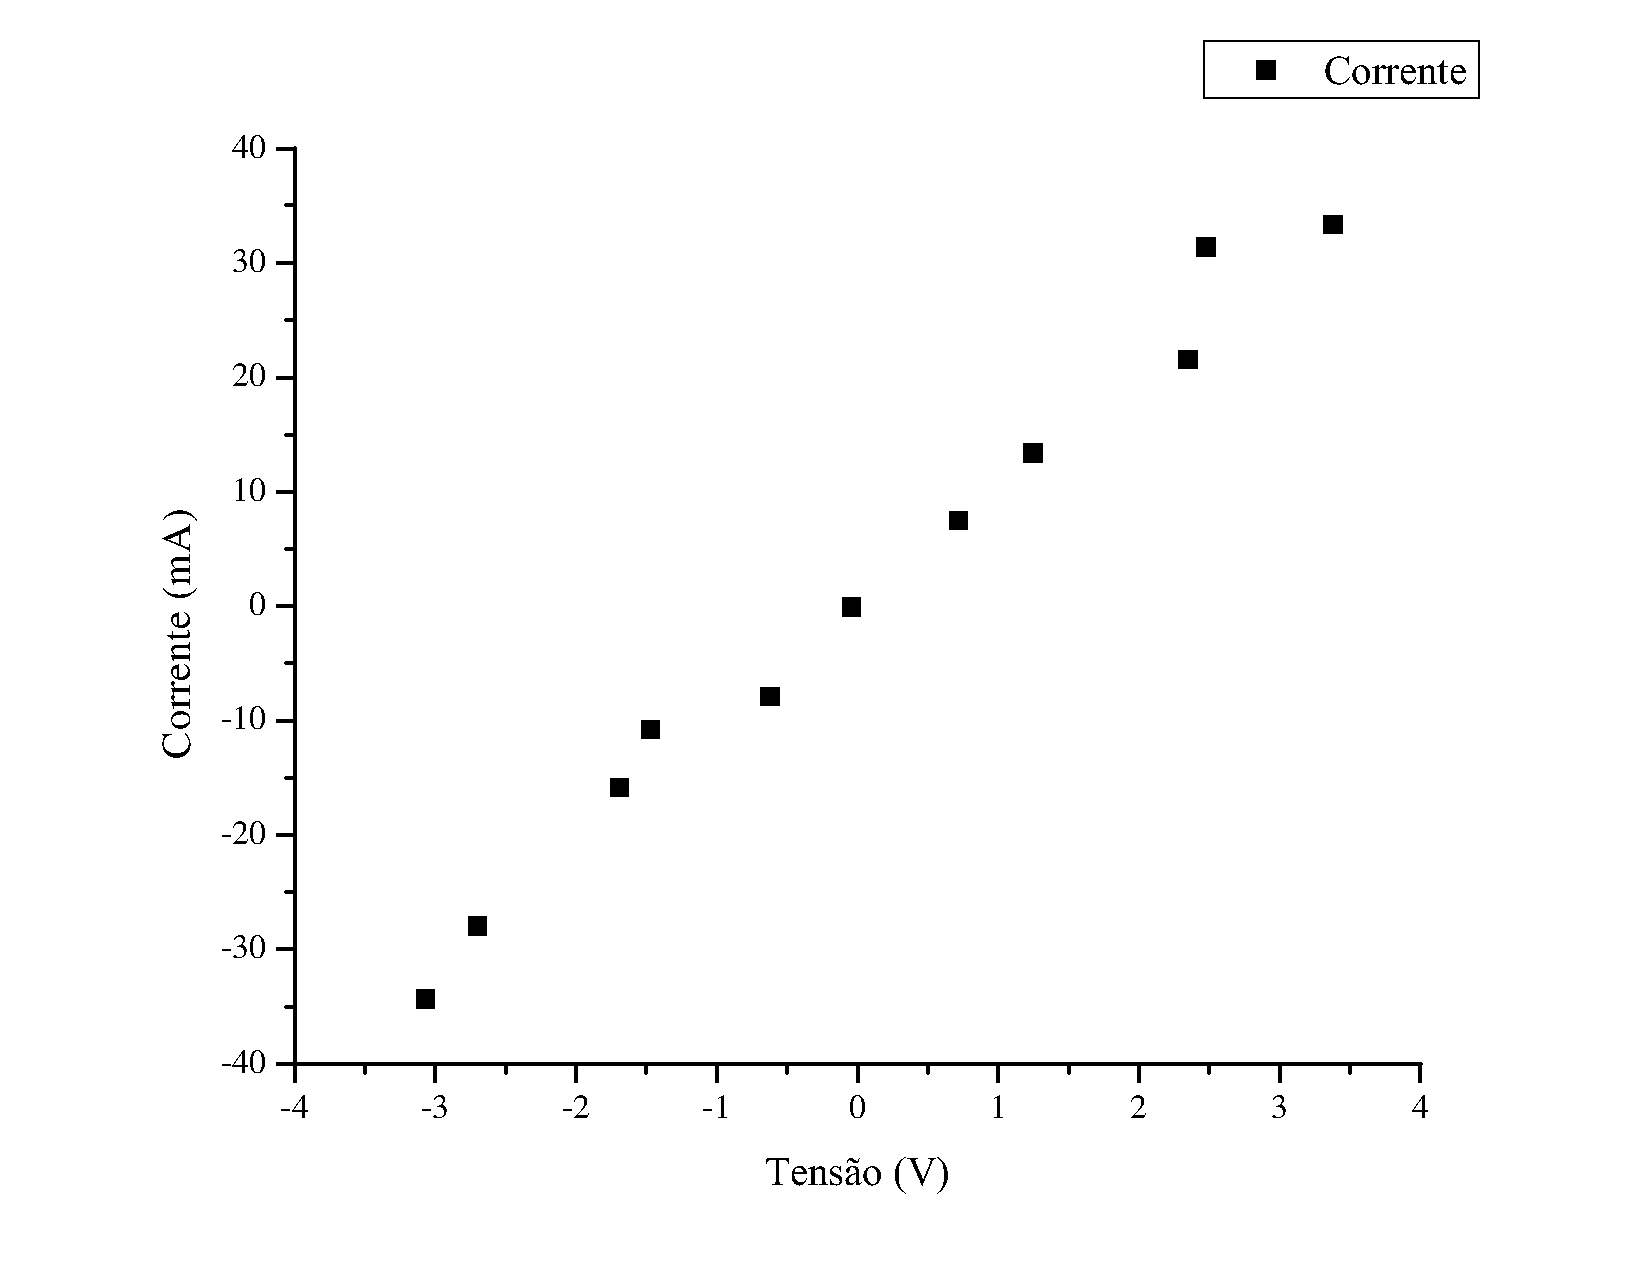
\includegraphics[width=0.8\textwidth]{reta/1linscatter.pdf}

        \caption{Resultado do \texttt{Scatter}}
        \label{fig:reta:linscatter}
    \end{figure}


\subsection{Tratamento da Legenda}

    O \texttt{Origin} gera uma legenda padrão para os elementos desenhados no gráfico. O ideal é alterá-las para serem mais informativas. As legendas também podem ser reposicionadas apenas arrastando-as.

    \begin{figure}[htbp]
        \centering
        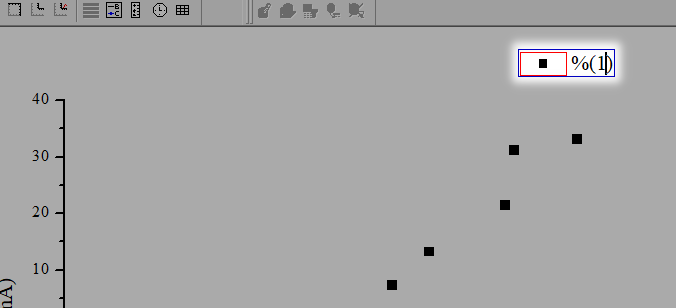
\includegraphics[width=0.8\textwidth]{reta/2legenda.png}

        \caption{Alterando o texto da legenda}
        \label{fig:reta:logenda}
    \end{figure}


\subsection{Marcadores de Ponto}

    Os pontos de dados do \texttt{Scatter} são por padrão marcados com um quadrado preenchido. Isso pode ser alterado acessando as opções por qualquer um dos pontos no gráfico. Existem várias opções de formatação do marcador, incluindo desenho, tamanho e cor.

    \begin{figure}[htbp]
        \centering
        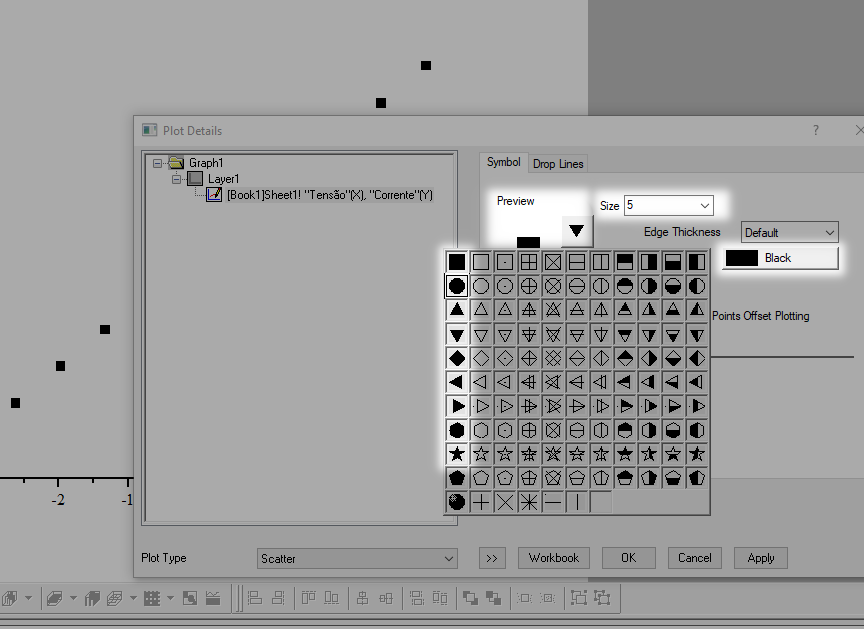
\includegraphics[width=0.8\textwidth]{reta/3marks.png}

        \caption{Alterando os marcadores}
        \label{fig:reta:marcadores}
    \end{figure}

    No material, será usado marcadores circulares, preenchidos com preto e de tamanho 5.


\subsection{Linhas de Grid}

    Para ler melhor os eixos do gráfico, é possível colocar retas acompanhando os valores principais.

    \begin{figure}[htbp]
        \centering
        \begin{subfigure}{0.25\textwidth}
            \centering
            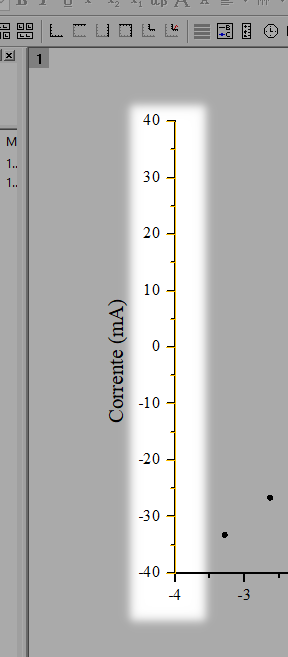
\includegraphics[width=\textwidth]{reta/4eixos.png}

            \caption{Acesso às opções dos eixos}
            \label{fig:reta:eixos}
        \end{subfigure}
        ~
        \begin{subfigure}{0.7\textwidth}
            \centering
            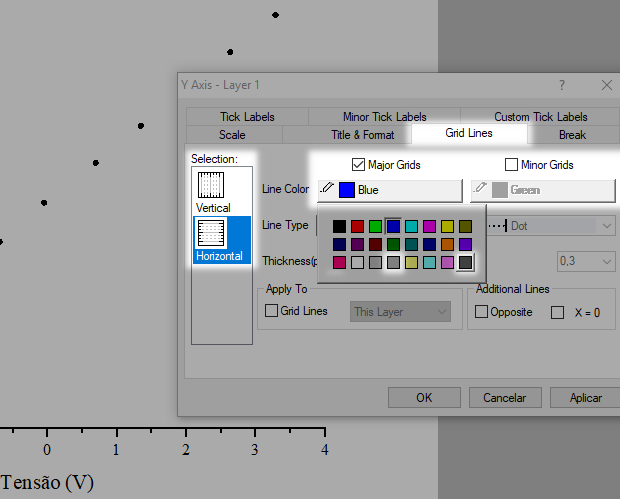
\includegraphics[width=\textwidth]{reta/5grid.png}

            \caption{Opções dos eixos (aba \texttt{Grid Lines})}
            \label{fig:reta:grid}
        \end{subfigure}
        \caption{Opções de linhas de \textit{grid}}
        \label{fig:reta:opcoes_eixo}
    \end{figure}

    No material, será utilizado linhas horizontais e verticais. As linhas principais serão em cinza escuro em traços e as linhas secundárias em cinza claro com pontilhado. Essas configurações podem e devem ser alteradas para cada gráfico, dependendo da importância da leitura dos valores.

    \begin{figure}[htbp]
        \centering
        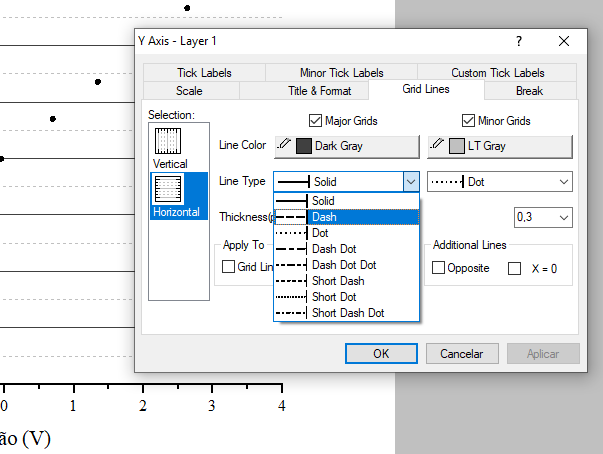
\includegraphics[width=0.8\textwidth]{reta/6gridtipo.png}

        \caption{Colocando e formatando as linha de acompanhamento dos eixos}
        \label{fig:reta:gridtipo}
    \end{figure}


\subsection{Resultado}

    \begin{figure}[htbp]
        \centering
        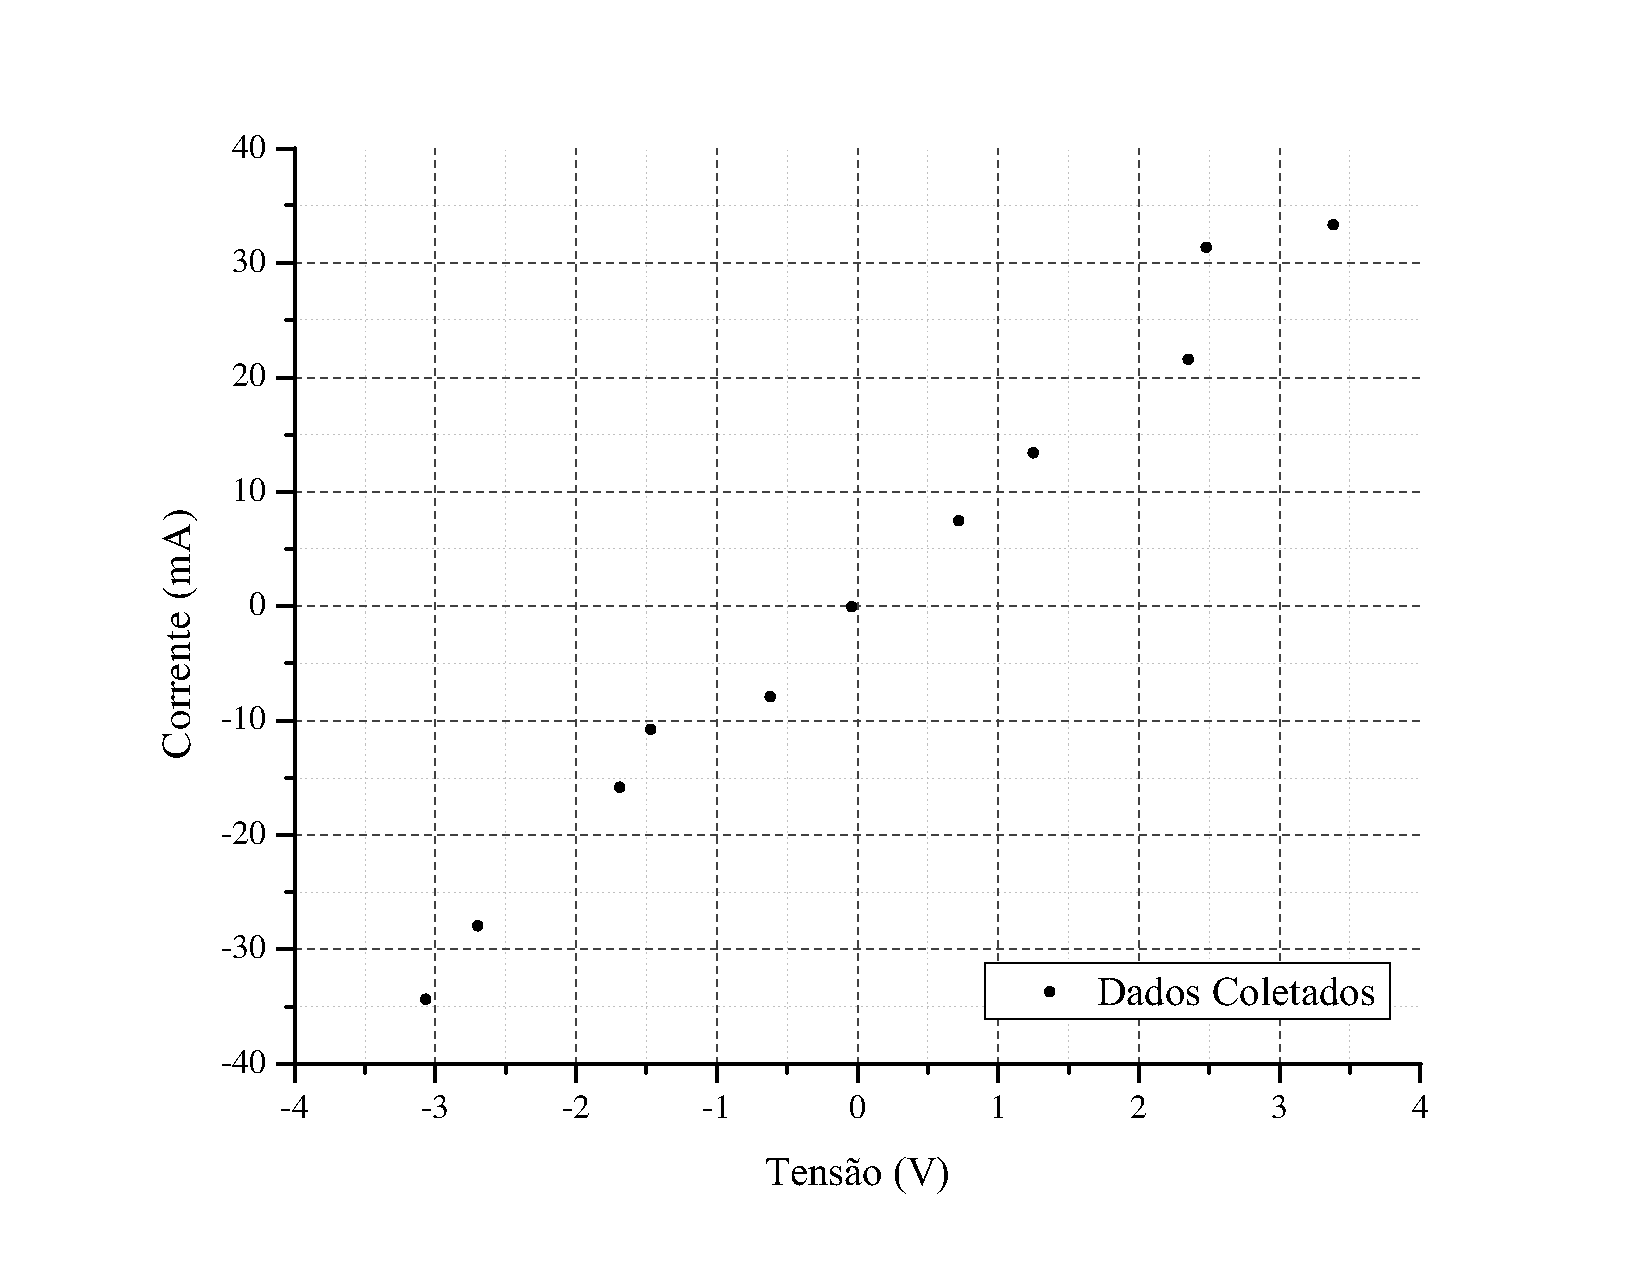
\includegraphics[width=0.8\textwidth]{reta/2gridlinscat.pdf}

        \caption{Gráfico de exemplo dos valores de corrrente e de tensão}
        \label{fig:reta:gridlinscat}
    \end{figure}

